%%%%%%%%%%%%%%%%%%%%%%%%%%%%%%%%%%%%%%%%%%
% labInstructions.cls provides all the styles needed
% us the option 'full' to show the solutions and
% additional assistant informations
%%%%%%%%%%%%%%%%%%%%%%%%%%%%%%%%%%%%%%%%%%
\documentclass[full]{labInstructions}

\title{{\Huge \scshape L'effet Cherenkov}\\{\Large Laboratoire PHYS-F-311}\\}
\date{}

\begin{document}

\maketitle

%%%%%%%%%%%%%%%%%%%%%%%%%%%%%%%%%%%%%%%%%%
% Introduction
%%%%%%%%%%%%%%%%%%%%%%%%%%%%%%%%%%%%%%%%%%
\section{Introduction}

Cette manipulation a pour but la caract\'erisation d'un module optique (OM) développé pour l'expérience AMANDA. Afin d'étidier les propriétés de cet OM, vous devrez mettre au point le dispositif nécéssaire à la prise de mesure. Après avoir pris connaissance avec le dispositif, vous serez ainsi amené à développer vous même la logique d'acquisition des données. Vous analyserez ensuite celle-ci grâce au outils statistiques et informatiques que vous aurez vous en cours. 

\pagebreak


%%%%%%%%%%%%%%%%%%%%%%%%%%%%%%%%%%%%%%%%%%
% Description of the experiments
%%%%%%%%%%%%%%%%%%%%%%%%%%%%%%%%%%%%%%%%%%
\section{Les dispositifs expérimentaux}
Dans cette section, nous allons introduire les deux dispositifs expérimentaux conçu pour la caractérisation des modules optiques (OMs) d'AMANDA.

\subsection{Dispositif 1: Effet Tcherenkov par des électrons}

Cette manipulation utilise une source de radiation $\beta^+$ composée de Strontium $^{90}$Sr. Les électrons émis par la source traverse ensuite une plaque de quartz d'indice de réfraction  $n = 1.478$. Lors de leur passage, les électrons vont produire un rayonnement Tcherenkov qui pourra être détecté par l'OM. Dans ce dispositif, l'OM se trouve à une position fixe située à un angle de 45$^{\circ}$ par rapport à la direction d'émission des électrons. La source radioactive est combinée à un spectromètre qui va nous permettre de sélectionner l'énergie cinétique des électrons afin de récolter un maximum de rayonnement Tcherenkov dans l'OM. Pour déterminer l'intensité du courant à fournir au spectromètre pour obtenir des électrons de cette énergie, vous devrez d'abord résoudre l'exercice 2.\\

Une fois cette valeur trouvée, vous pouvez allumer le spectromètre. Ce spectromètre est calibré sur la partie descendante de la courbe d'hystérèse, il vous faudra donc respecter les conditions d'utilisations décrites ci-dessous.\\

\textbf{Mode d'emploi du spectromètre :}
\begin{quote}
    \begin{itemize}
        \item Démarrez à $I$ = 0 A
        \item Aller à saturation $I$ $\sim$ 2,6 A
        \item Descendre à la valeur $I_t$ désirée
    \end{itemize}
\end{quote}
\textbf{Remarque :} Si on veut changer $I_t$ pour une valeur plus petite, on descend vers cette valeur. En revanche, si on veut augmenter cette valeur, on doit recommencer le cycle d'hystérèse. 

\begin{figure}[!h]
    \center{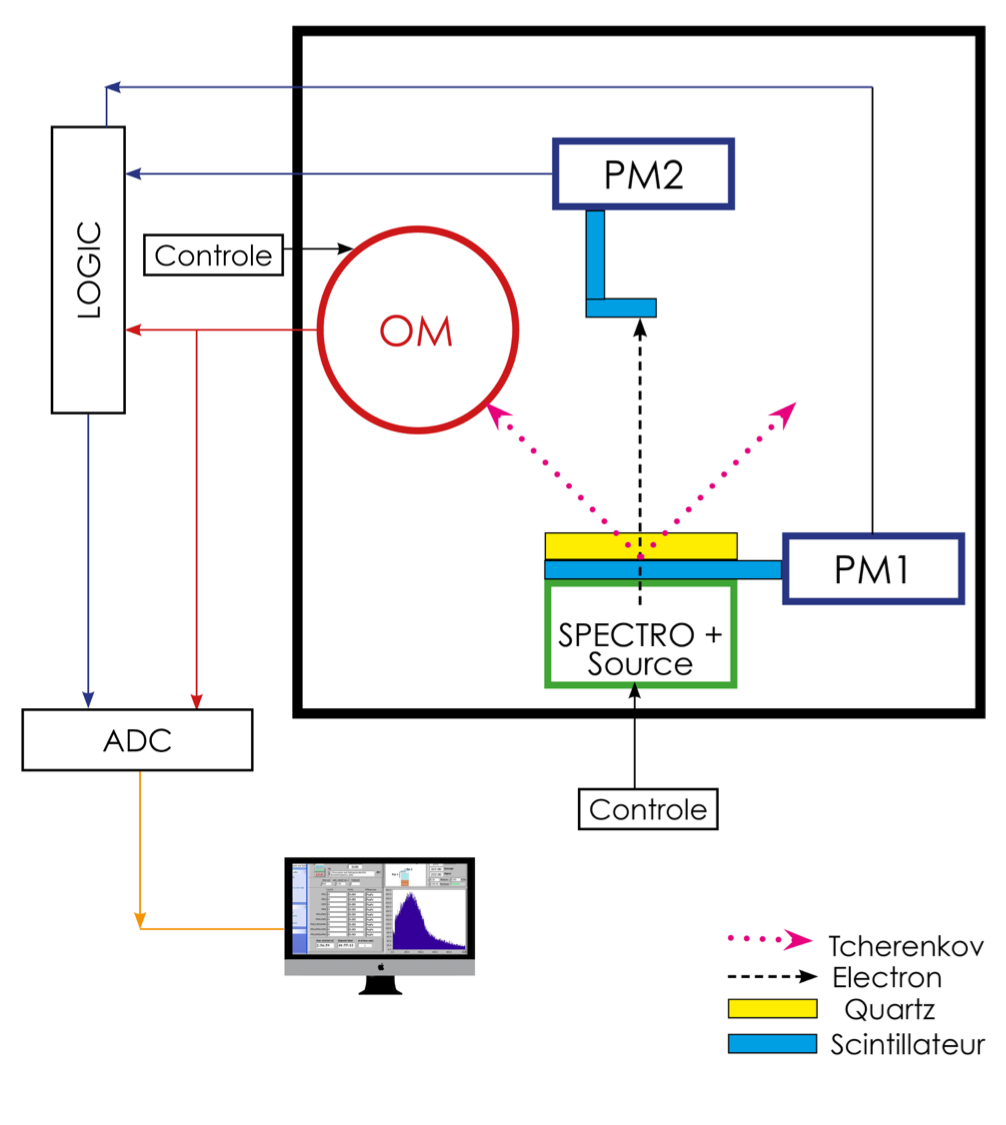
\includegraphics[width=0.5\textwidth]
    {figures/Dispositif_1.png}}
    \caption{\label{fig:dispo1} Dispositif expérimental de l'effet Tcherenkov produit par des électrons.}
\end{figure}

Dans ce dispositif, sont également présent 2 photo-multiplicateurs (PMs) chacun relié à un scintillateur. Le premier (PM1) est situé entre la source et la plaque de quartz et nous permet de vérifier qu'un électron a été émis par la source. Le second PM confirme que l'électron a bien traversé le quartz. Ces PMs ont donc pour but d'assurer que le signal détecté par l'OM est en coïncidence avec un électron qui a produit des photons Tcherenkov.

\subsection{Dispositif 2: Effet Tcherenkov par des muons}

Pour cette seconde manipulation, nous utilisons les muons atmosphériques afin d'obtenir l'émission Tcherenkov. Ce dispositif est composé de 4 scintillateurs chacun relié à un photo-multiplicateur (PM), d'un OM, une couche de plomb et d'un réservoir d'eau. Ce réservoir forme un angle de 45$^{\circ}$ avec la verticale. Les trois premiers PM (PM1, PM2 et PM3) assure la direction verticale du muon incident. La présence d'une couche de plomb avant le PM3 nous permet également de vérifier que le muon est suffisamment énergétique pour produire le rayonnement Tcherenkov avec l'angle souhaité. Un 4ème PM est placé au dessus de l'OM et est utilisé comme veto. Puisque les muons sont produits en "paquets", appelés muon bundles, ce veto exclu les évènements de l'OM qui seraient produits par un second muon plutôt que par un photon Tcherenkov.


\begin{figure}[!h]
    \center{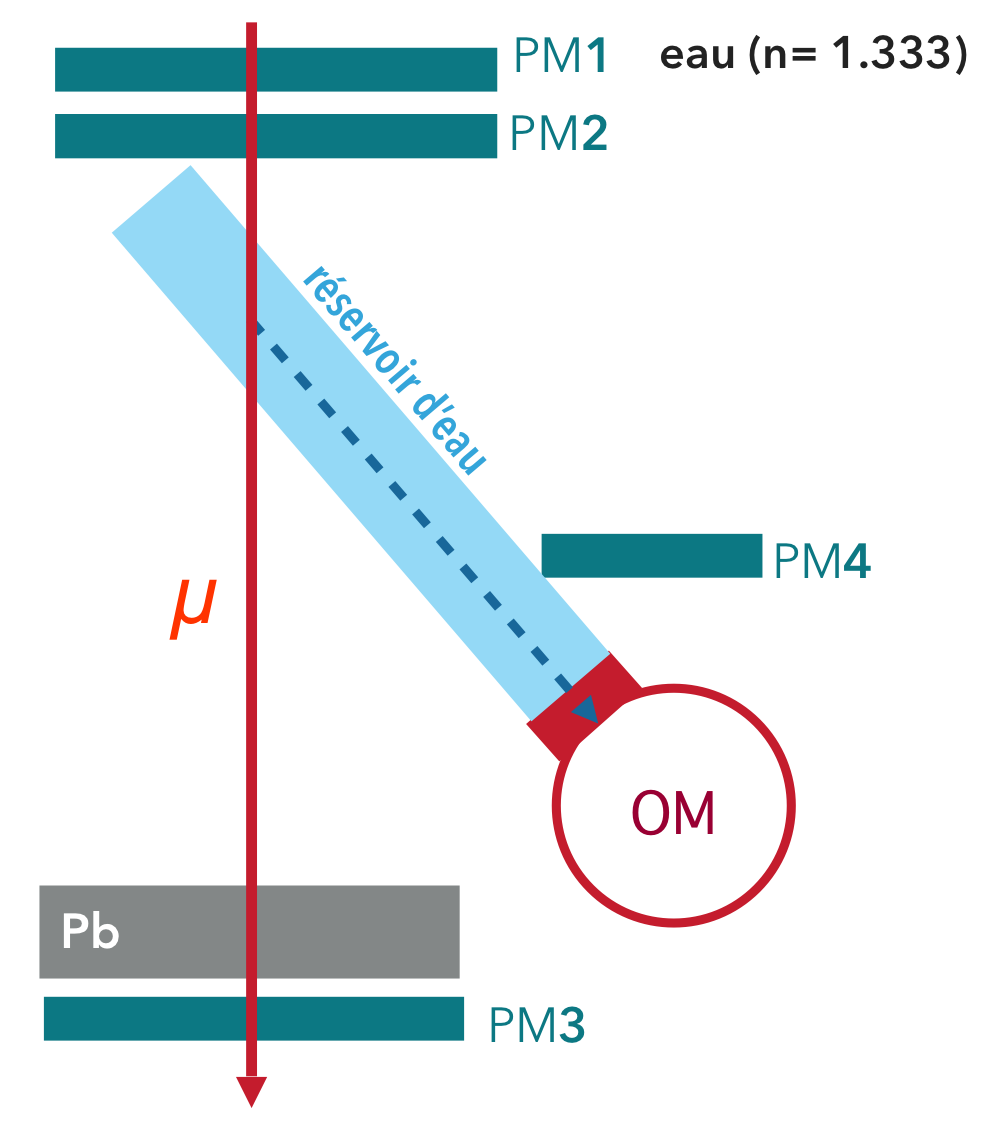
\includegraphics[width=0.5\textwidth]
    {figures/Dispositif_2.png}}
    \caption{\label{fig:dispo2} Dispositif expérimental de l'effet Tcherenkov produit par des muons.}
\end{figure}


\subsection{Le matériel expérimental}


\pagebreak

%%%%%%%%%%%%%%%%%%%%%%%%%%%%%%%%%%%%%%%%%%
% Exercises
%%%%%%%%%%%%%%%%%%%%%%%%%%%%%%%%%%%%%%%%%%
\section{Exercices Pr\'eparatoires}

\subsection{Exercice 1}
Pour le 2\`eme dispositif, calculez quelle sera l'angle d'\'emission du rayonnement Cherenkov \'emis dans l’eau par des muons ($m_\mathrm{\mu} = 0.106$\,GeV/$c^2$) de $1.5$\,GeV/$c$ de quantit\'e de mouvement, sachant que l'indice de r\'efraction de l'eau \`a $20^\circ$C est $1.333$.

\ifthenelse{\boolean{showAdditional}}{
\begin{additional}
\begin{align*}
\begin{split}
\beta &= \frac{v}{c} = \frac{pc}{E}\\
 &= \frac{pc}{\sqrt{p^2c^2+m_\mathrm{\mu}^2c^4}}\\
 &= 0.9975\\
\end{split}
\quad
\begin{split}
\cos\Theta_\mathrm{c} &= \frac{1}{\beta n}\\
 \Theta_\mathrm{c} &= \arccos\frac{1}{0.9975\cdot1.33}\\
 &= \boxed{41.2^\circ} 
\end{split}
\end{align*}
\end{additional}
}

\subsection{Exercice 2}
Pour le 1er dispositif, sachant que l'OM est plac\'e \`a un angle de $45^\circ$ par rapport \`a la direction d'\'emission des \'electrons ($m_\mathrm{e} = 0.511$\,MeV/$c^2$) de la source de strontium, \`a quel courant faut-il r\'egler le spectrom\`etre pour r\'ecolter un maximum de rayonnement Cherenkov dans l'OM, sachant que l'indice de r\'efraction du quartz est de $1.478$?

\ifthenelse{\boolean{showAdditional}}{
\begin{additional}
\begin{align*}
\beta &= \frac{1}{n\cos\Theta_\mathrm{c}} = 0.9568\\
 &= \frac{pc}{E}\\
 &= \frac{\sqrt{E^2-m_\mathrm{e}^2c^4}}{E}\\
 &\\
E &= \sqrt{\frac{m_\mathrm{e}^2c^4}{1 - \beta^2}} = 1.7575\,\mathrm{MeV}\\
E_\mathrm{cin}&=E- m_\mathrm{e}\\
 &= 1.247\,\mathrm{MeV} \\
&\Rightarrow \boxed{I \approx 950\,\mathrm{mA}} \\
\end{align*}
\end{additional}
}

\subsection{Exercice 3}
Pour le 1er dispositif, calculer l'ordre de grandeur du nombre de photons \'emis entre $350$ et $500$\,nm par un 'electron de $1247$\,keV d'\'energie cin\'etique traversant une fen\^etre de quartz de 1\,mm d'\'epaisseur, sachant que pour ce domaine de longueurs d’onde, l'indice de r\'efraction du quartz varie de moins de 1\% et peut \^etre consid\'er'e constant ($1.478$). N\'egliger la perte d'\'energie de l'\'electron dans le quartz.\\ $\alpha = 1/137$

\ifthenelse{\boolean{showAdditional}}{
\begin{additional}
Formule de \emph{Frank-Tamm}:
\begin{align*}
\frac{\mathrm{d}N}{\mathrm{d}x} &= \int_{\lambda_0}^{\lambda_1} \frac{2\pi\alpha z^2}{\lambda^2} \sin^2\Theta_\mathrm{c} \mathrm{d}\lambda\\
&=\frac{\pi}{137}\int_{350\,\mathrm{nm}}^{500\,\mathrm{nm}}\frac{\mathrm{d}\lambda}{\lambda^2}\\
N&=\frac{\pi}{137}\cdot\left(\frac{1}{350\,\mathrm{nm}}-\frac{1}{500\,\mathrm{nm}}\right)\cdot1\,\mathrm{mm}\\
&=\boxed{19.65}
\end{align*}
\end{additional}
}

\subsection{Exercice 4}
En supposant que le diam\`etre du collimateur plac\'e devant la photocathode de l'OM est de 6 cm et qu'il se trouve \`a 17\,cm de la fen\^etre de quartz, combien de photoelectrons l'OM peut-il enregistrer par \'electron de la source, en supposant la transmittance $T$ \`a 90\%, l'efficacit\'e quantique est de $\epsilon_\mathrm{q}=15\%$?

\ifthenelse{\boolean{showAdditional}}{
\begin{additional}
Avec $N_\mathrm{\gamma}^{\mathrm{quartz}}$ trouv\'e avant, on obtient:
\begin{align*}
N_{\mathrm{pe}} &= \epsilon_\mathrm{q} \cdot T \cdot N_\mathrm{\gamma}^{\mathrm{OM}}\\
 &= \epsilon_\mathrm{q} \cdot T \cdot \frac{6\,\mathrm{cm}}{2\pi \cdot 17\,\mathrm{cm} \cdot\sin\Theta_\mathrm{c}} \cdot N_\mathrm{\gamma}^{\mathrm{quartz}}\\
&= \boxed{3.58}
\end{align*}
\end{additional}
}

\pagebreak


%%%%%%%%%%%%%%%%%%%%%%%%%%%%%%%%%%%%%%%%%%
% Analysis
%%%%%%%%%%%%%%%%%%%%%%%%%%%%%%%%%%%%%%%%%%
\section{Prise de donn\'ees}

Pour cette manipulation, il vous est demandé de pr\'eparer le dispositif expérimental n\'ecessaire à la prise de mesure. Cela implique :

\begin{center}
\fbox{
\begin{minipage}{0.75\textwidth}
Dans un premier temps, de se familiariser avec le dispositif :
\begin{itemize}
\item \'etudier l'efficacit\'e des PMs,
\item calibrer l'ADC,
\item d\'evelopper la logique d'aquisition de donn\'ees.
\end{itemize}
\end{minipage}
}
\end{center}


\subsection{Mesure de l'efficacit\'e}

Il vous est demandé de mesurer l'efficacit\'e d'un des photo-multiplicateurs (PM) présents dans votre dispositif. Vous devrez faire cette mesure en faisant varier dans un premier temps le seuil du PM pour lequel vous mesurer l'efficacit\'e. Une fois la valeur optimale du seuil trouv\'ee, r\'epetez le processus en faisant cette fois varier la tension appliquée sur le PM en question. Pour ces deux mesures, veillez également à mesurer le taux d'\ev\`enements d\'etect/'es par le PM dont vous mesurez l'efficacit\'e.

\ifthenelse{\boolean{showAdditional}}{
\begin{additional}

\textbf{Dispositif muon :}
\begin{quote}
\begin{itemize}
\item Mesure de l'efficacite du PM2
\item Logique d'acquisition : PM1&PM2&PM3 - PM1&PM3
\item Mesure du rate du PM2
\end{itemize}
\end{quote}


\textbf{Dispositif \'electron :}
\begin{quote}
\begin{itemize}
\item Mesure de l'efficacite du PM1
\item Logique d'acquisition : PM1&PM2&OM - PM2&OM
\item Mesure du rate du PM1
\end{itemize}
\end{quote}
}

\subsection{Calibration de l'ADC}

Nous allons \`a pr\'esent proc\'eder \`a la calibration de l'ADC. 

\section{Analyse de donn\'ees}

A pr\'esent, nous pouvons nous concentrer sur l'analyse des donn\'ees dans le but de caract\'eriser l'OM.

En vous basant sur les donn\'ees, vous devrez calculer :
\begin{center}
\fbox{
\begin{minipage}{0.75\textwidth}
\textbf{Dispositif muon :}
\begin{quote}
\begin{itemize}
\item le gain $G$ de l'OM,
\item la r\'esolution $\sigma_\mathrm{G}$ de l'OM,
\item le nombre moyen de photo-\'electrons $\langle n_{\mathrm{pe}}\rangle$ produit par trigger dans l'OM.
\end{itemize}
\end{minipage}
}
\end{center}



\end{center}
\pagebreak


\end{document}
